\section{Auswertung}

\subsection{Überprüfung der Proportionalität zwischen der Leuchtfleckverschiebung und der Ablenkspannung \label{sec:empf}}

Die aufgenommenen Messwerte für die Beschleunigungsspannungen $U_B = \SI{210}{\V}$, $U_B = \SI{250}{\V}$, $U_B = \SI{290}{\V}$,
$U_B = \SI{320}{\V}$ und $U_B = \SI{350}{\V}$ befinden sich in Tabelle \ref{tab:messges}.
\begin{table}[H]
   \centering
   \caption{Messwerte zur Bestimmung der Empfindlichkeit der Kathodenstrahlröhre}
   \label{tab:messges}
   \begin{tabular} { S S S S S S }
 \toprule
 {$D\:/\: \mathrm{cm}$} & {$U_{210}\:/\: \mathrm{V}$} & {$U_{250}\:/\: \mathrm{V}$} &
 {$U_{290}\:/\: \mathrm{V}$} & {$U_{320}\:/\: \mathrm{V}$} & {$U_{350}\:/\: \mathrm{V}$} \\
    \midrule
    0,0 & -21,3 & -25,5 & -29,1 & -32,0 & -34,5 \\
    0,6 & -17,0 & -20,6 & -24,1 & -26,3 & -28,3 \\
    1,2 & -13,3 & -16,2 & -18,4 & -21,1 & -22,5 \\
    1,8 & -9,8 & -11,8 & -13,7 & -15,0 & -16,2 \\
    2,4 & -6,3 & -7,1 & -8,3 & -9,7 & -10,6 \\
    3,0 & -2,4 & -2,5 & -3,4 & -4,1 & -4,1 \\
    3,6 & 1,5 & 2,0 & 1,5 & 2,0 & 2,1 \\
    4,2 & 5,4 & 6,5 & 6,1 & 7,8 & 8,0 \\
    4,8 & 9,1 & 11,0 & 11,9 & 13,4 & 14,3 \\
    \bottomrule
  \end{tabular}
\end{table}


\newpage
Diese sind in Abbildung \ref{fig:empf} dargestellt.
\begin{figure}[H]
  \centering
  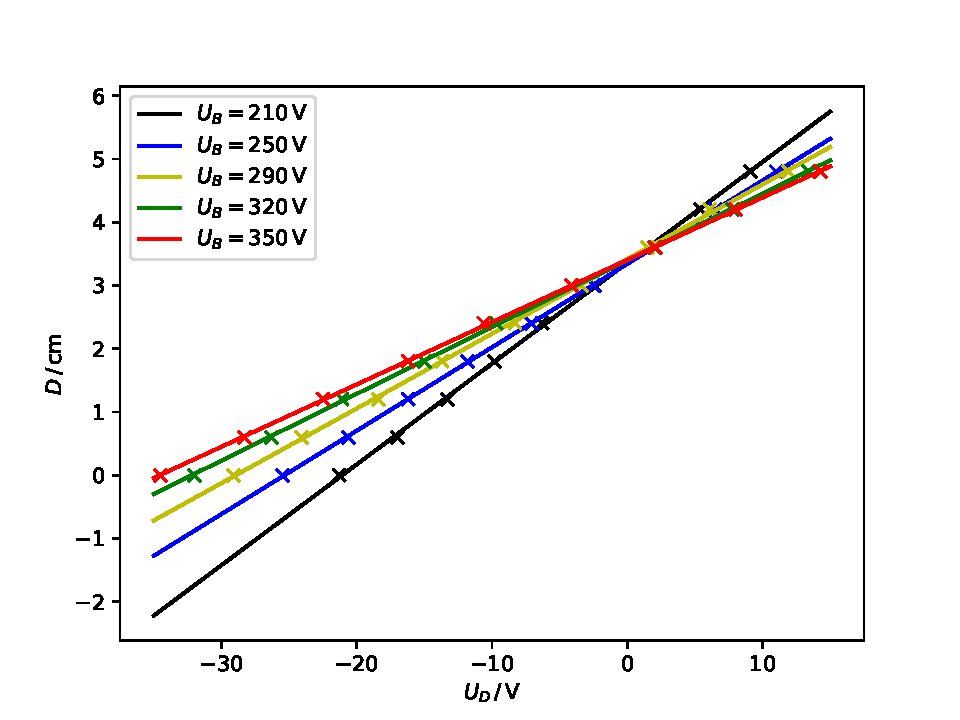
\includegraphics[width=\textwidth]{Plots/empf.pdf}
  \caption{$D$-$U_d$-Diagramm zur Bestimmung der Empfindlichkeiten der Kathodenstrahlröhre}
  \label{fig:empf}
\end{figure}

Die lineare Regression $f(x) = a \cdot x + b$ ergibt
\begin{align*}
  a_{210} &= \SI{1,594(12)}{\milli \meter \per \volt}\\
  a_{250} &= \SI{1,319(4)}{\milli \meter \per \volt}\\
  a_{290} &= \SI{1,181(9)}{\milli \meter \per \volt}\\
  a_{320} &= \SI{1,055(6)}{\milli \meter \per \volt}\\
  a_{350} &= \SI{0,985(4)}{\milli \meter \per \volt}\\
\end{align*}

\newpage
Diese Empfindlichkeiten werden in Abbildung \ref{fig:konst} aufgetragen.
\begin{figure}[H]
  \centering
  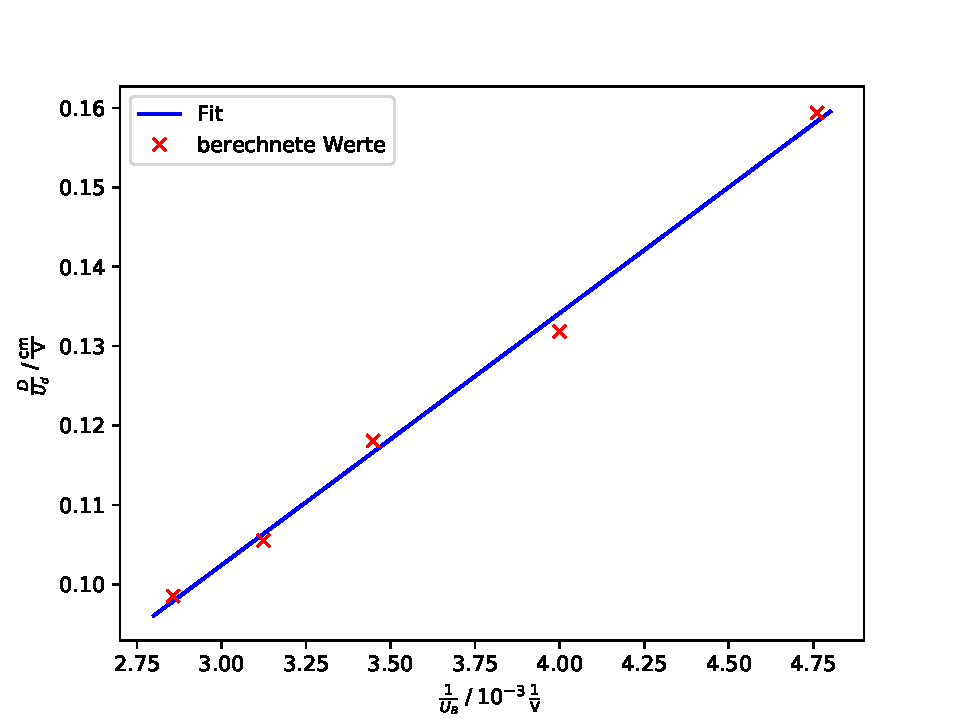
\includegraphics[width=\textwidth]{Plots/konst.pdf}
  \caption{Diagramm zur Bestimmung der Apparaturkonstante $k$}
  \label{fig:konst}
\end{figure}

Eine erneute lineare Regression ergibt die Steigung
\begin{equation*}
  a = \SI{31,74(40)}{\cm} = k
\end{equation*}

Der Theoriewert ergibt sich aus
\begin{equation}
  k_\text{theo} = \frac{p L}{2 d} = \SI{21,9}{\cm}.
\end{equation}

Die Abweichung beträgt $44,91 \%$. Die benötigten Werte werden der Versuchsanleitung entnommen.

\newpage

\subsection{Bestimmung der Signalspannung mithilfe eines Kathodenstrahl-Oszillographen}

Die aufgenommenen Messwerte befinden sich in Tabelle \ref{tab:oszi}.
\begin{table}[H]
   \centering
   \caption{Aufgenommene Sägezahnfrequenzen und daraus resultierende Signalfrequenzen}
   \label{tab:oszi}
   \begin{tabular} { c S S }
 \toprule
 {$n$} & {$\nu_\text{Säg}\:/\: \mathrm{Hz}$} & {$\nu_\text{Sig}\:/\: \mathrm{Hz}$} \\
    \midrule
    1/4 & 19,95 & 79,80 \\
    1/3 & 26,62 & 79,86 \\
    1/2 & 39,91 & 79,82 \\
    1 & 79,87 & 79,87 \\
    \bottomrule
  \end{tabular}
\end{table}


Gemittelt nach \eqref{eqn:mit} und \eqref{eqn:sta}
\begin{align}
  \bar{x} &= \frac{1}{N} \sum_{i=1}^{N} x_i
  \label{eqn:mit} \\
  \Delta \bar{x} &= \sqrt{\frac{1}{N (N - 1)} \sum_{i=1}^{N} (x_i - \bar{x})^2}.
  \label{eqn:sta}
\end{align}

beträgt die Signalspannung $\bar{\nu}_\text{Sig} = \SI{79,84(2)}{\Hz}$.
Der Scheitelwert $S$ errechnet sich aus der Empfindlichkeit und der gemessenen Strahlauslenkung $\SI{1,5}{\cm}$ zu $S = \SI{18,27}{\V}$.

\subsection{Bestimmung der spezifischen Ladung $\sfrac{e_0}{m_0}$ \label{sec:spez}}

Die aufgenommenen Messwerte für die Beschleunigungsspannungen $U_B = \SI{250}{\V}$ und $U_B = \SI{400}{\V}$ befinden sich
in Tabelle \ref{tab:mag}.
\begin{table}[H]
   \centering
   \caption{Messwerte zur Bestimmung der spezifischen Ladung}
   \label{tab:mag}
   \begin{tabular} { S S S }
 \toprule
 {$D\:/\: \mathrm{cm}$} & {$I_{250}\:/\: \mathrm{A}$} & {$I_{400}\:/\: \mathrm{A}$} \\
    \midrule
    0,0 & 0,00 & 0,00 \\
    0,6 & 0,30 & 0,45 \\
    1,2 & 0,60 & 0,90 \\
    1,8 & 0,90 & 1,30 \\
    2,4 & 1,25 & 1,70 \\
    3,0 & 1,60 & 2,15 \\
    3,6 & 1,90 & 2,60 \\
    4,2 & 2,25 & 3,10 \\
    4,5 &  & 3,25 \\
    4,8 & 2,55 &  \\
    \bottomrule
  \end{tabular}
\end{table}


Mithilfe von Gleichung \eqref{eqn:bfeld}
\begin{equation}
  B = \mu_0 \frac{8}{\sqrt{125}} \frac{N I}{R}
  \label{eqn:bfeld}
\end{equation}

werden die Magnetfelder aus den Spulenströmen aus Tabelle \ref{tab:mag} berechnet. Die benötigten Werte sind
\begin{align*}
  N &= 20 \\
  R &= \SI{0,282}{\m}
\end{align*}

Daraus ergibt sich Abbildung \ref{fig:mag}.
\begin{figure}[H]
  \centering
  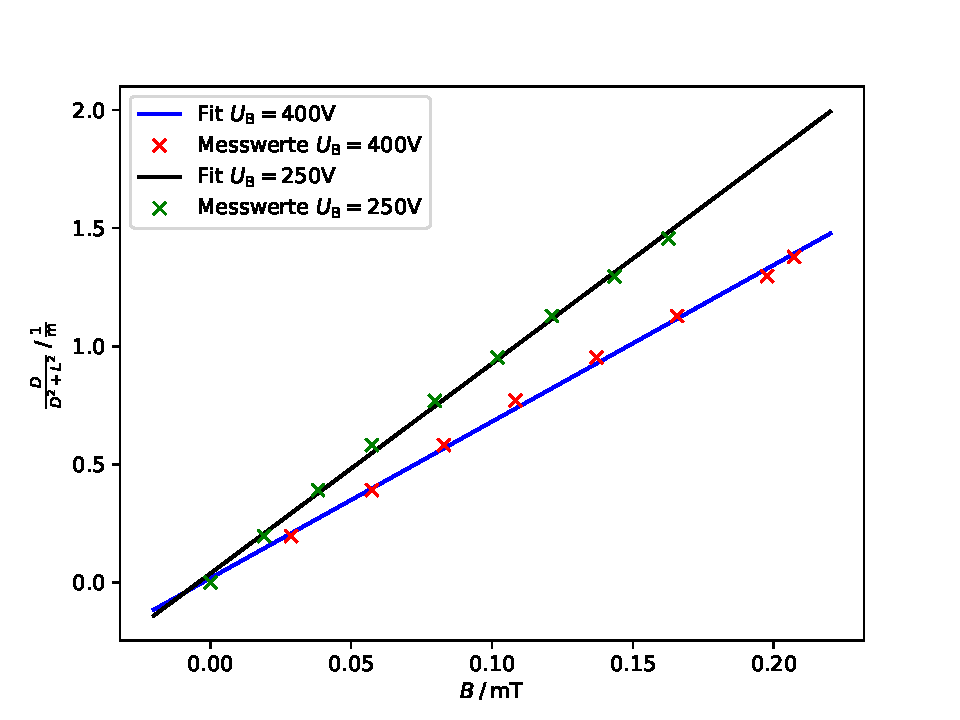
\includegraphics[width=\textwidth]{Plots/magnet.pdf}
  \caption{Diagramm zur Bestimmung der spezifischen Ladung}
  \label{fig:mag}
\end{figure}

Die lineare Regression $f(x) = a \cdot x + b$ ergibt
\begin{align*}
  a_{250} = \SI{8,89(16)e3}{\per \tesla \per \meter} \\
  a_{400} = \SI{6,63(11)e3}{\per \tesla \per \meter}
\end{align*}

Mithilfe von Gleichung \eqref{eqn:spez}
\begin{equation}
  \frac{e_0}{m_0} = 8 a^2 U_b
  \label{eqn:spez}
\end{equation}

ergeben sich folgende Werte für die spezifische Ladung
\begin{align*}
  \left(\frac{e_0}{m_0}\right)_{250} &= \SI{1,58e11}{\coulomb \per \kg} \\
  \left(\frac{e_0}{m_0}\right)_{400} &= \SI{1,41e11}{\coulomb \per \kg}
\end{align*}

Gemittelt nach \eqref{eqn:mit} und \eqref{eqn:sta} erhält man
\begin{equation*}
\left(\frac{e_0}{m_0}\right)_{\!\!\diameter} = \SI{1,49(9)e11}{\coulomb \per \kg}.
\end{equation*}

Die Abweichung vom Theoriewert \cite{scipy} $\left(\frac{e_0}{m_0}\right)_\text{theo}=\SI{1,76e11}{\coulomb \per \kg}$ beträgt $15,05 \%$.

\subsection{Bestimmung des Erdmagnetfeldes}

Der gemessene Gegenstrom beträgt $I = \SI{0,2}{\A}$ und der Inklinationswinkel $\varphi = \SI{70}{°}$.
Mithilfe des Inklinationswinkels $\varphi$ und von Gleichung \eqref{eqn:bfeld} berechnet sich das totale Magnetfeld zu
\begin{equation*}
  B_\text{total} = 37,29 \, \symup{\mu T} .
\end{equation*}
